% Szglab4
% ===========================================================================
%
\chapter{Analízis modell kidolgozása 2}

\thispagestyle{fancy}

\section{Objektum katalógus}

\subsection{\bf Simulation}
%Szimuláció objektum. A szimulációért felelős. Elindítja a jelgenerátor léptetőt, s utasítja az áramkört %több kiértékelési ciklus lefuttatásához, amíg az áramkörben van változás. Ha a változás megadott lépésen %belül nem áll meg, tájékoztatja a felhasználót, hogy nincs stacionárius állapot. Amikor leállítódik, a %jelgenerátor-léptetőt is leállítja.
A szimulációért felelős objektum. Létrehozza a szimulálni kívánt áramkört. Utasítja az áramkört több kiértékelési ciklus lefuttatásához, amíg az áramkörben van változás. Ha a változás megadott lépés szám limiten belül nem áll meg, tájékoztatja a felhasználót, hogy nincs stacionárius állapot.

\subsection{\bf State}
A szimuláció állapotát megvalósító objektum. 3 állapotot különböztetünk meg:
\begin{itemize}
\item a szimuláció fut \item a szimuláció sikeresen lefutott \item a szimuláció során hiba történt
\end{itemize}

\subsection{\bf Circuit}
%Az áramkör objektum. Ezen objektum feladata a jelgenerátor léptető kérésére a jelgenerátorok léptetése, %az áramkörben található komponensek utasítása arra, hogy töröljék a "már kiértékelve" flaget egy adott %kiértékelési ciklus előtt, hogy ezáltal a ciklusban minden kimenet értéke frissülhessen.
%Továbbá feladata a kiértékelés elindítása az összes kijelzőre, mert a rendszer kiértékelése a kijelzők %kiértékelésével kezdődik.
Az áramkör objektum. Ez az objektum hozza létre és köti össze egymással az áramköri elemeket. Törli az egyes elemek "már kiértékelt" flagjét a kiértékelési ciklus előtt, hogy ezáltal a ciklusban minden kimenet értéke frissülhessen. További feladata a kiértékelés elindítása az összes kijelzőre, mert a rendszer kiértékelése a kijelzők kiértékelésével kezdődik. A flip-flopokat utasítja arra, hogy mentsék el a jelenlegi kimenetüket belső állapotként és az órajel bemenetén lévő értéket az éldetektálás érdekében. Megmondja, hogy az áramköri elemek értékei megváltoztak-e. Ezen kívül lépteti a jelgenerátorokat.

\subsection{\bf SequenceGenerator}
Jelgenerátor, az áramkört felépítő egyik alapelem, kiértékelési kezdeményezés hatására az előre betáplált jelsorozat éppen aktuális elemét adja ki a kimenetén. Nincs áramköri bemenete. Mikor az áramkör kéri tőle, hogy lépjen, akkor a bitsorozat következő elemét fogja kiadni kimenetén.

\subsection{\bf Value}
A logikai értékeket megvalósító objektum. Jelenleg két érték lehetséges: logikai igaz, logikai hamis.

\subsection{\bf AndGate}
ÉS kapu, az áramkör egyik alapeleme. Bemeneteire kötött komponensek kiértékelését kezdeményezi, s a kapott értékek logikai ÉS kapcsolatát valósítja meg, melynek eredményét a kimenetén kiadja.

\subsection{\bf OrGate}
VAGY kapu, az áramkör egyik alapeleme. Bemeneteire kötött komponensek kiértékelését kezdeményezi, s a kapott értékek logikai VAGY kapcsolatát valósítja meg, melynek eredményét a kimenetén kiadja.

\subsection{\bf Inverter}
Invertáló, az áramkör alapelemei közé tartozik. A bemenetére érkező jel logikai negáltját valósítja meg, amit a kimenetén kiad.

\subsection{\bf Gnd}
Föld, az áramkört felépítő egyik elem, állandó értéke logikai hamis. Bemenete nem létezik, így nem kezdeményez további kiértékeléseket.

\subsection{\bf Vcc}
Tápfeszültség, az áramkör egyik alapeleme, mely állandóan a logikai igazt adja ki a kimenetén.

\subsection{\bf Led}
Egy kijelző, az áramkör alapeleme, bemenetére kötött komponens kiértékelését kezdeményezi, és ezáltal az aktuális értékét egy a felhasználó számára érzékelhető módon kijelzi.

\subsection{\bf Toggle}
Kapcsoló, az áramkör egyik eleme, melynek aktuális értéke állítható, ez jelenik meg a kimenetén. Áramköri bemenete nincs.

\subsection{\bf FlipFlopD}
D flip flopot megvalósító objektum. Csak akkor lép működésbe, mikor az órajelbemenetén a logikai érték hamisról igazra változik, ekkor az értékbemenettől függően változtatja a kimeneti értékét.

\subsection{\bf FlipFlopJK}
JK flip flopot megvalósító objektum. Csak akkor lép működésbe, mikor az órajelbemenetén a logikai érték hamisról igazra változik, ekkor az értékbemenetektől és a belső állapotától függően változtatja a kimeneti értékét.

\subsection{\bf Mpx}
4-1-es multiplexer áramköri építőelemet megvalósító objektum. Bemeneteire kötött komponensek kiértékelését kezdeményezi, a választó bemenet függvényében adja ki a kimeneten az egyik, vagy másik értékbemenetére kötött értéket.

\subsection{\bf SevenSegmentDisplay}
Hétszegmenses kijelző objektuma. Minden bemenete egy-egy szegmensért felelős, melyek 8-as alakban helyezkednek el, és a bemenetre kötött érték függvényében világítanak.

\section{Osztályok leírása}

\subsection{AbstractComponent}
Absztrakt osztály.
\begin{itemize}
\item Felelősség\\
Egy komponens absztrakt megvalósítása, ebből származik az összes többi  komponens. A közös logikát valósítja meg. A gyakran használt feladatokra ad alapértelmezett implementációt (összekötés, bemenetek kiértékelése stb.). Tudja magáról, hogy kiértékelték-e már az adott áramköri kiértékelési ciklusban, illetve, hogy a legutóbbi két kiértékelés között változtak-e a kimenetei.
\item Ősosztályok: (nincs)
\item Interfészek: (nincs)
\item Attribútumok $\ $
\begin{itemize}
	\item \texttt{protected Value[] values}: Kimeneteken lévő értékek. Ez frissül az \texttt{evaluate()} meghívására, ha még nem volt kiértékelve.
	\item \texttt{protected AbstractComponent[] inputs}: A bemenetekre kötött komponensek.
\end{itemize}
\item Metódusok$\ $
\begin{itemize}
	\item \texttt{addTo(Circuit c)}: Meghívja az áramkör \texttt{add(AbstractComponent ac)} metódusát.
	\item \texttt{Value[] evaluate()}: Komponens kimenetein lévő értékek újraszámolása (ha még nem volt kiértékelve) a bemenetek alapján. A kimeneteken lévő értékekkel tér vissza.
	\item \texttt{void clearEvaluatedFlag()}: Töröljük a komponens "kiértékelt" flagjét.
	\item \texttt{boolean isChanged()}: Visszaadja, hogy a legutóbbi két kiértékelés között változtak-e a kimenetek.
	\item \raggedright \texttt{void setInput(int inputPin, AbstractComponent component, int outputPin)}: Beállítunk egy bemenetet (adott bemeneti lábra rákötjük az adott komponens adott kimeneti lábát).
\end{itemize}
\end{itemize}

\subsection{AndGate}
\begin{itemize}
\item Felelősség\\
ÉS kapu, az áramkör egyik alapeleme. Bemeneteire kötött értékeken a logikai ÉS műveletet hajtva végre, és ennek eredményét adja ki a kimenetén.
\item Ősosztályok:\ AbstractComponent
\item Interfészek: (nincs)
\item Attribútumok $\ $
\begin{itemize}
\item (nincs)
\end{itemize}
\item Metódusok$\ $
\begin{itemize}
\item (nincs)
\end{itemize}
\end{itemize}

\subsection{Circuit}
\begin{itemize}
\item Felelősség\\
A komponensek létrehozása és összekötése a szimuláció elején, szimuláció által indított kiértékelési ciklus végrehajtása. Rajta keresztül léptethetőek a jelgenerátorok és véglegesíthető a FF-ok állapota.
\item Ősosztályok: (nincs)
\item Interfészek: (nincs)
\item Attribútumok $\ $
\begin{itemize}
	\item \texttt{private Collection<AbstractComponent> components}: Összes áramköri komponens
	\item \texttt{private Collection<DisplayComponent> displays}: Megjelenítő típusú komponensek (kijelző, 7-szegmenses kijelző)
	\item \texttt{private Collection<SourceComponent> sources}: Jelforrás típusú komponensek (kapcsoló, jelgenerátor)
	\item \texttt{private Collection<FlipFlop> flipFlops}: Flipflopok (D és JK flipflopok)
	\item \texttt{private Collection<SequenceGenerator> sequenceGens}: Jelgenerátorok
\end{itemize}
\item Metódusok$\ $
\begin{itemize}
	\item \texttt{void init()}: Áramkör inicializálása; komponensek létrehozása és összekötése.
	\item \texttt{void add(AbstractComponent component)}: Komponens hozzáadása a \texttt{components}-hez. Ezt minden komponensre meg kell hívni.
	\item \raggedright \texttt{void add(SourceComponent sc)}: Jelforrás hozzáadása a \texttt{sources}-hoz és az \texttt{add(AbstractComponent component)} meghívása.
	\item \raggedright \texttt{void add(FlipFlop ff)}: FlipFlop hozzáadása a \texttt{flipFlops}-hoz és az \texttt{add(AbstractComponent component)} meghívása.
	\item \raggedright \texttt{void add(SequenceGenerator sg)}: Jelgenerátor hozzáadása a \texttt{sequenceGens}-hez és az \texttt{add(AbstractComponent component)} meghívása.
	\item \raggedright \texttt{void add(DisplayComponent dc)}: Megjelenítő hozzáadása a \texttt{displays}-hez és az \texttt{add(AbstractComponent component)} meghívása.
	\item \texttt{void doEvaluationCycle()}: Egy kiértékelési ciklus lefuttatása. Az áramkörtől ezután lekérdezhető, hogy változott-e a rendszer állapota, azaz valamelyik komponens eltérő kimenetet ad-e, mint az előző ciklusban.
	\item \texttt{boolean isChanged()}: Áramkör változásának lekérdezése. Igazzal tér vissza, ha van olyan komponens, ami azt jelzi magáról, hogy változott a kimenete az előző kiértékeléshez képest.
	\item \texttt{void commitFlipFlops()}: A flipflopok jelenlegi kimenetének elmentése belső állapotnak, és az órajel bemenetén lévő érték eltárolása az éldetektálás érdekében.
	\item \texttt{void stepGenerators()}: Jelgenerátorok léptetése.
\end{itemize}
\end{itemize}

\subsection{DisplayComponent}
Absztrakt osztály.
\begin{itemize}
\item Felelősség\\
Megjelenítő típusú komponensek ősosztálya.
\item Ősosztályok:\ AbstractComponent.
\item Interfészek: (nincs).
\item Attribútumok $\ $
\begin{itemize}
	\item (nincs)
\end{itemize}
\item Metódusok$\ $
\begin{itemize}
\item \texttt{addTo(Circuit c)}: Meghívja az áramkör \texttt{add(DisplayComponent dc)} metódusát.
\end{itemize}
\end{itemize}

\subsection{FlipFlop}
Absztrakt osztály.
\begin{itemize}
\item Felelősség\\
Flipflopok ősosztálya, itt vannak leírva a flipflopok közös logikája.
\item Ősosztályok:\ AbstractComponent
\item Interfészek: (nincs)
\item Attribútumok $\ $
\begin{itemize}
\item (nincs)
%	\item \texttt{protected Value q}: A flip-flopban tárolt érték (az előző állapot)
%	\item \texttt{protected Value clk}: A rendszer előző stabil állapotánál mért flip-flop órajel-bemenetére érkező érték (ennek segítségével tudunk detektálni élváltozást).
\end{itemize}
\item Metódusok$\ $
\begin{itemize}
	\item \texttt{addTo(Circuit c)}: Meghívja az áramkör \texttt{add(FlipFlop ff)} metódusát.
	\item \texttt{void commit()}: Az FF jelenlegi kimenetét és az órajel bemenetét elmenti. Előbbivel frissítjük a belső állapotot, utóbbi pedig az éldetektáláshoz kell. Ezt akkor kell meghívni, amikor az áramkör az adott áramköri bemenetekre stabil állapotba ért.
	\item \texttt{boolean isActive()}: Számolhat-e az FF? Ezt kell ellenőrizniük a konkrét flipflop implementációknak, hiszen ekkor kellhet a belső állapottól eltérő állapotot kiadni.
\end{itemize}
\end{itemize}

\subsection{FlipFlopD}
\begin{itemize}
\item Felelősség\\
D flipflop, mely felfutó órajelnél beírja a belső állapotába az adatbemeneten lévő értéket. Kimenetén a belső állapota jelenik meg.
\item Ősosztályok:\ AbstractComponent $\rightarrow{}$ FlipFlop.
\item Interfészek: (nincs)
\item Attribútumok $\ $
\begin{itemize}
\item (nincs)
\end{itemize}
\item Metódusok$\ $
\begin{itemize}
\item (nincs)
\end{itemize}
\end{itemize}

\subsection{FlipFlopJK}
\begin{itemize}
\item Felelősség\\
JK flipflop, mely felfutó órajelnél a Követelmények résznél leírt módon a J és K bemenetén lévő értéktől és belső állapotától függően változtatja a belső állapotát. Kimenetén a belső állapota jelenik meg.
\item Ősosztályok:\ AbstractComponent $\rightarrow{}$ FlipFlop.
\item Interfészek: (nincs)
\item Attribútumok $\ $
\begin{itemize}
\item (nincs)
\end{itemize}
\item Metódusok$\ $
\begin{itemize}
\item (nincs)
\end{itemize}
\end{itemize}

\subsection{Gnd}
\begin{itemize}
\item Felelősség\\
A "föld" komponens, mely állandóan a hamis értéket adja ki. Nincs bemenete.
\item Ősosztályok:\ AbstractComponent.
\item Interfészek: (nincs)
\item Attribútumok $\ $
\begin{itemize}
\item (nincs)
\end{itemize}
\item Metódusok$\ $
\begin{itemize}
\item (nincs)
\end{itemize}
\end{itemize}

\subsection{Inverter}
\begin{itemize}
\item Felelősség\\
Inverter alkatrész, mely invertálva adja ki a kimenetén a bemenetén érkező jelet.
\item Ősosztályok:\ AbstractComponent.
\item Interfészek: (nincs)
\item Attribútumok $\ $
\begin{itemize}
\item (nincs)
\end{itemize}
\item Metódusok$\ $
\begin{itemize}
\item (nincs)
\end{itemize}
\end{itemize}

\subsection{Led}
\begin{itemize}
\item Felelősség\\
Egy LED-et reprezentál, mely világít, ha bemenetén igaz érték van.
\item Ősosztályok:\ AbstractComponent $\rightarrow{}$ DisplayComponent.
\item Interfészek: (nincs)
\item Attribútumok $\ $
\begin{itemize}
\item (nincs)
\end{itemize}
\item Metódusok$\ $
\begin{itemize}
	\item \texttt{Value getValue()}: Visszaadja a bemenetére kötött értéket.
\end{itemize}
\end{itemize}

\subsection{Mpx}
\begin{itemize}
\item Felelősség\\
4-1-es multiplexer, amely 4 adatbemenettel, 2 kiválasztó-bemenettel és 1 kimenettel rendelkezik. A kiválasztó-bemenetekre adott értéktől függ, hogy melyik adatbemenet értéke jelenik meg az adatkimeneten.
\item Ősosztályok:\ AbstractComponent.
\item Interfészek: (nincs)
\item Attribútumok $\ $
\begin{itemize}
\item (nincs)
\end{itemize}
\item Metódusok$\ $
\begin{itemize}
\item (nincs)
\end{itemize}
\end{itemize}

\subsection{OrGate}
\begin{itemize}
\item Felelősség\\
VAGY kapu, az áramkör egyik alapeleme. Bemeneteire kötött értékeken a logikai VAGY műveletet hajtva végre, és ennek eredményét adja ki a kimenetén.
\item Ősosztályok:\ AbstractComponent.
\item Interfészek: (nincs)
\item Attribútumok $\ $
\begin{itemize}
\item (nincs)
\end{itemize}
\item Metódusok$\ $
\begin{itemize}
\item (nincs)
\end{itemize}
\end{itemize}

\subsection{SequenceGenerator}
\begin{itemize}
\item Felelősség\\
Jelgenerátort reprezentál, amely a beállított bitsorozatot adja ki.
\item Ősosztályok:\ AbstractComponent $\rightarrow{}$ SourceComponent.
\item Interfészek: (nincs)
\item Attribútumok $\ $
\begin{itemize}
	\item \texttt{private int index}: A bitsorozat egy indexe, ez határozza meg, hogy éppen melyik értéket adja ki a kimenetén.
	\item \texttt{private Value[] sequence}: Tárolt bitsorozat
\end{itemize}
\item Metódusok$\ $
\begin{itemize}
\item \texttt{addTo(Circuit c)}: Meghívja az áramkör \texttt{add(SequenceGenerator sg)} metódusát.
	\item \texttt{Value[] getValues()}: Jelgenerátor bitsorozatának lekérdezése
	\item \texttt{void setValues(Value[] values)}: Jelgenerátor bitsorozatának beállítása
	\item \texttt{void step()}: A jelgenerátor lép, a bitsorozat következő elemére ugrik. A következő léptetésig ez kerül kiadásra a kimeneteken.
\end{itemize}
\end{itemize}

\subsection{SevenSegmentDisplay}
\begin{itemize}
\item Felelősség\\
7-szegmenses kijelzőt reprezentál, melynek 7 bemenete vezérli a  megfelelő szegmenseket, ezek világítanak, ha az adott bemenetre logikai igaz van kötve.
\item Ősosztályok:\ AbstractComponent $\rightarrow{}$ DisplayComponent.
\item Interfészek: (nincs)
\item Attribútumok $\ $
\begin{itemize}
\item (nincs)
\end{itemize}
\item Metódusok$\ $
\begin{itemize}
	\item \texttt{Value getSegment(int idx)}: Visszaadja az adott szegmenshez tartozó bemenetre kötött értéket.
\end{itemize}
\end{itemize}

\subsection{Simulation}
\begin{itemize}
\item Felelősség\\
Az áramkörön kiértékelési ciklusok futtatása az adott áramkör bemenetekre (kapcsolók állapota, jelgenerátorok jelenlegi értéke) nézve addig, amíg az áramkör nem stabilizálódik.
\item Ősosztályok: (nincs)
\item Interfészek: (nincs)
\item Attribútumok $\ $
\begin{itemize}
	\item \texttt{private Circuit circuit}: Szimulált áramkör
\end{itemize}
\item Metódusok$\ $
\begin{itemize}
	\item \texttt{boolean start()}: Szimuláció elindítása a jelenlegi áramköri bemenetekre (kapcsolók állapota, jelgenerátorok jelenlegi értéke). Amennyiben stacionárius állapot jött létre, léptetjük a jelgenerátorokat és elmentjük a flipflopok állapotát. Így újbóli hívásra már a következő időpillanatban érvényes áramköri bemenetekre lehet szimulálni az áramkört. A visszatérési érték a sikerességet jelzi (sikertelen, ha nincs stacionárius állapot).
	\item \texttt{State getState(State state)}: Szimuláció állapotának lekérdezése.
\end{itemize}
\end{itemize}

\subsection{Simulation.State}
Enumeráció.
\begin{itemize}
\item Felelősség\\
Szimuláció állapotait írja le
\item Ősosztályok: (nincs)
\item Interfészek: (nincs)
\item Attribútumok $\ $
\begin{itemize}
	\item \texttt{public static final State READY} A szimuláció kész a futásra. Ilyenkor hívható rajta a start() metódus.
	\item \texttt{public static final State WORKING} Szimuláció éppen dolgozik, egy konkrét jelforrás-kombinációt alkalmazva szimulálja az áramkört.
	\item \texttt{public static final State FAILED} A szimuláció leállt, mert az áramkörnek nincs stacionárius állapota. A start() metódus újra hívható (ha a bemenetek nem változnak, továbbra is le fog állni).
\end{itemize}
\item Metódusok$\ $
\begin{itemize}
\item (nincs)
\end{itemize}
\end{itemize}

\subsection{SourceComponent}
Absztrakt osztály.
\begin{itemize}
\item Felelősség\\
Jelforrás típusú komponensek ősosztálya.
\item Ősosztályok:\ AbstractComponent.
\item Interfészek: (nincs).
\item Attribútumok $\ $
\begin{itemize}
	\item (nincs)
\end{itemize}
\item Metódusok$\ $
\begin{itemize}
\item \texttt{addTo(Circuit c)}: Meghívja az áramkör \texttt{add(SourceComponent dc)} metódusát.
	\item \texttt{abstract Value[] getValues()}: Lekérhetjük a jelforrás értékeit. Ennek megvalósítása a konkrét implementációk feladata.
	\item \texttt{abstract setValues(Value[] values)}: Beállítjuk a jelforrás értékét. Ennek megvalósítása a konkrét implementációk feladata. (pl. kapcsoló csak 1 elemű tömböt kaphat)
\end{itemize}
\end{itemize}





\subsection{Toggle}
\begin{itemize}
\item Felelősség\\
Kapcsoló jelforrás, melynek két állapota lehet; egyikben logikai igazat, másikban logikai hamist ad ki.
\item Ősosztályok:\ AbstractComponent $\rightarrow{}$ SourceComponent.
\item Interfészek: (nincs)
\item Attribútumok $\ $
\begin{itemize}
\item (nincs)
\end{itemize}
\item Metódusok$\ $
\begin{itemize}
	\item \texttt{Value[] getValues()}: Lekérjük a kapcsoló értékét (1 elemű tömb)
	\item \texttt{void setValues(Value[] values)}: Kapcsoló állapotának változtatása, csak 1 elemű tömböt kaphat paraméterül.
\end{itemize}
\end{itemize}

\subsection{Value}
Enumeráció.
\begin{itemize}
\item Felelősség\\
Az áramkörben előfordulható értéket reprezentál.
\item Ősosztályok: (nincs)
\item Interfészek: (nincs)
\item Attribútumok $\ $
\begin{itemize}
	\item \texttt{public static final Value FALSE} 
 % TODO
	\item \texttt{public static final Value TRUE} 
 % TODO
\end{itemize}
\item Metódusok$\ $
\begin{itemize}
	\item \texttt{Value invert()}: Invertálja az adott értéket. Ennek addig van értelme, amíg 2 féle  állapot fordulhat elő a rendszerben.
\end{itemize}
\end{itemize}

\subsection{Vcc}
\begin{itemize}
\item Felelősség\\
A tápfeszültés komponens, ami konstans igaz értéket ad. Nincs bemenete.
\item Ősosztályok:\ AbstractComponent.
\item Interfészek: (nincs)
\item Attribútumok $\ $
\begin{itemize}
\item (nincs)
\end{itemize}
\item Metódusok$\ $
\begin{itemize}
\item (nincs)
\end{itemize}
\end{itemize}

\section{Statikus struktúra diagramok}

\begin{figure}[H]
\begin{center}
\includegraphics*[angle=90, width=17cm, viewport = 25 30 695 565]{chapters/chapter04/classdiagram/class.pdf}
\caption{Statikus struktúra nézet}
\label{fig:class_diagram}
\end{center}
\end{figure}
%
%\begin{figure}[H]
%\begin{center}
%\includegraphics*[angle=90, width=14cm, viewport = 765 475 1530 930]{chapters/chapter03/classdiagram/class_diagram.pdf}
%\caption{Statikus struktúra nézet (jobb felső)}
%\label{fig:class_diagram}
%\end{center}
%\end{figure}
%
%\begin{figure}[H]
%\begin{center}
%\includegraphics*[angle=90, width=14cm, viewport = 0 0 765 475]{chapters/chapter03/classdiagram/class_diagram.pdf}
%\caption{Statikus struktúra nézet (bal alsó)}
%\label{fig:class_diagram}
%\end{center}
%\end{figure}
%
%\begin{figure}[H]
%\begin{center}
%\includegraphics*[angle=90, width=14cm, viewport = 765 0 1530 475]{chapters/chapter03/classdiagram/class_diagram.pdf}
%\caption{Statikus struktúra nézet (jobb alsó)}
%\label{fig:class_diagram}
%\end{center}
%\end{figure}

\section{Szekvencia diagramok}

\begin{figure}[H]
\begin{center}
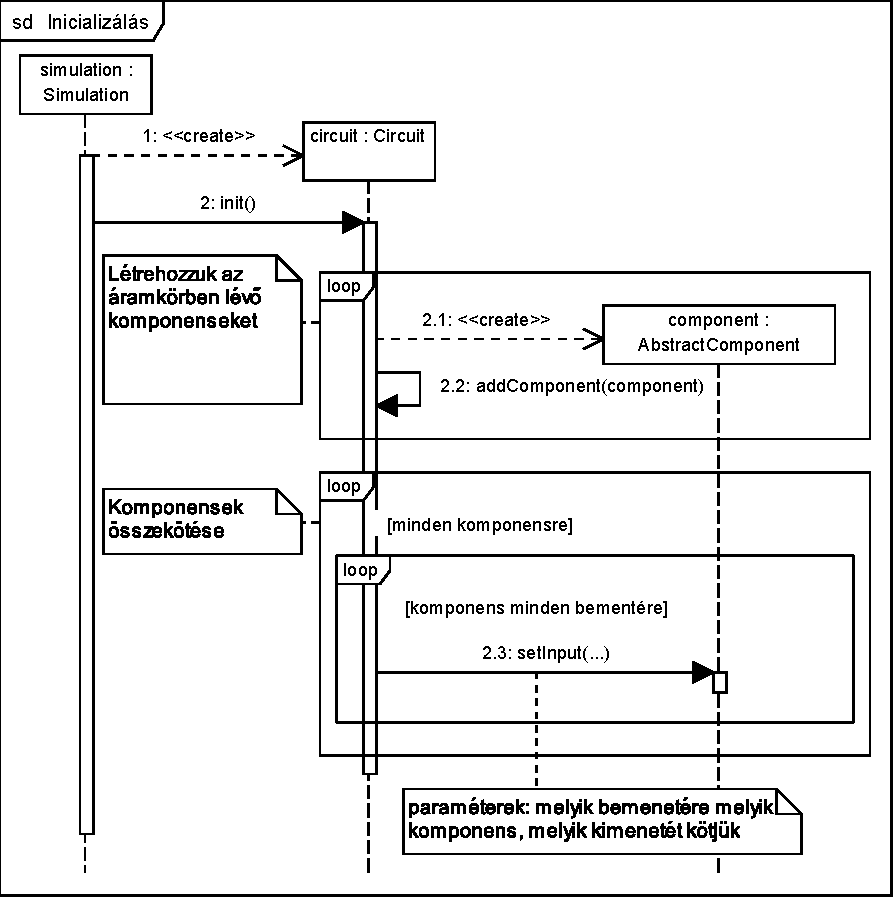
\includegraphics{chapters/chapter04/seqdiagrams/new/init.pdf}
\caption{Inicializálás}
\label{fig:init}
\end{center}
\end{figure}

\begin{figure}[H]
\begin{center}
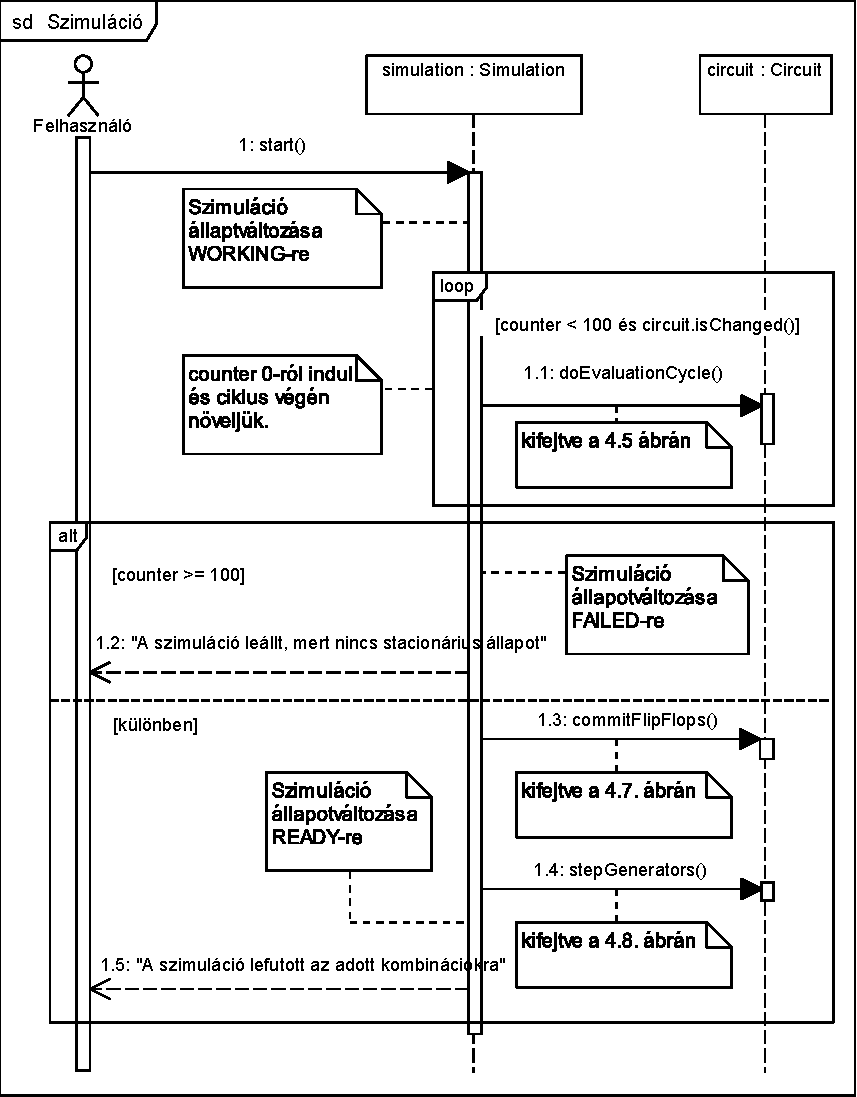
\includegraphics{chapters/chapter04/seqdiagrams/new/simulation.pdf}
\caption{Szimuláció}
\label{fig:simulation}
\end{center}
\end{figure}

%\begin{figure}[H]
%\begin{center}
%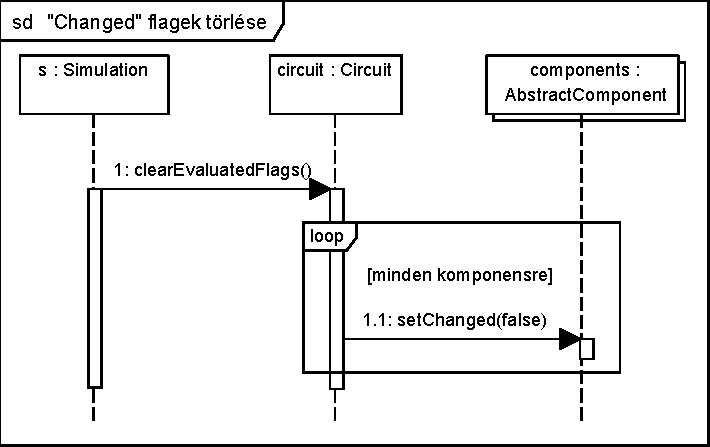
\includegraphics{chapters/chapter04/seqdiagrams/clear_changed_flags.pdf}
%\caption{"Changed" flag-ek törlése}
%\label{fig:clear_changed_flags}
%\end{center}
%\end{figure}

\begin{figure}[H]
\begin{center}
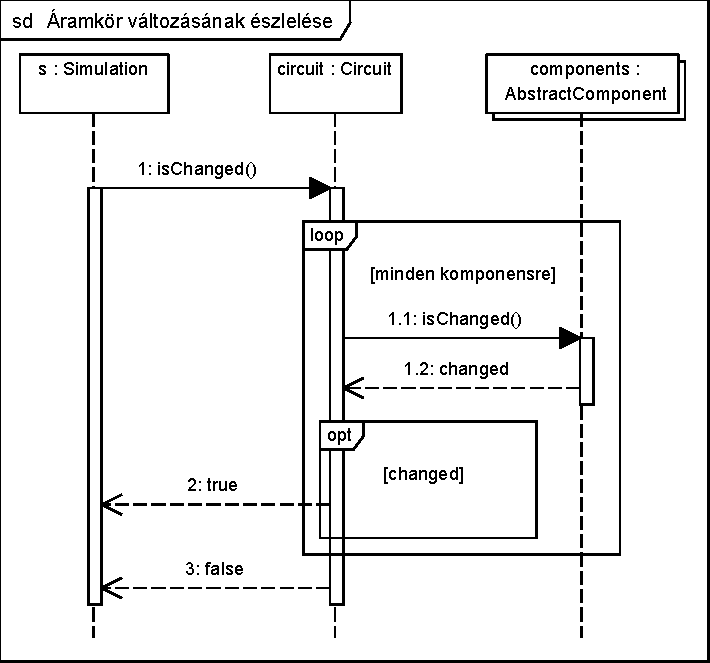
\includegraphics{chapters/chapter04/seqdiagrams/is_changed.pdf}
\caption{Áramkör változásának észlelése}
\label{fig:is_changed}
\end{center}
\end{figure}

\begin{figure}[H]
\begin{center}
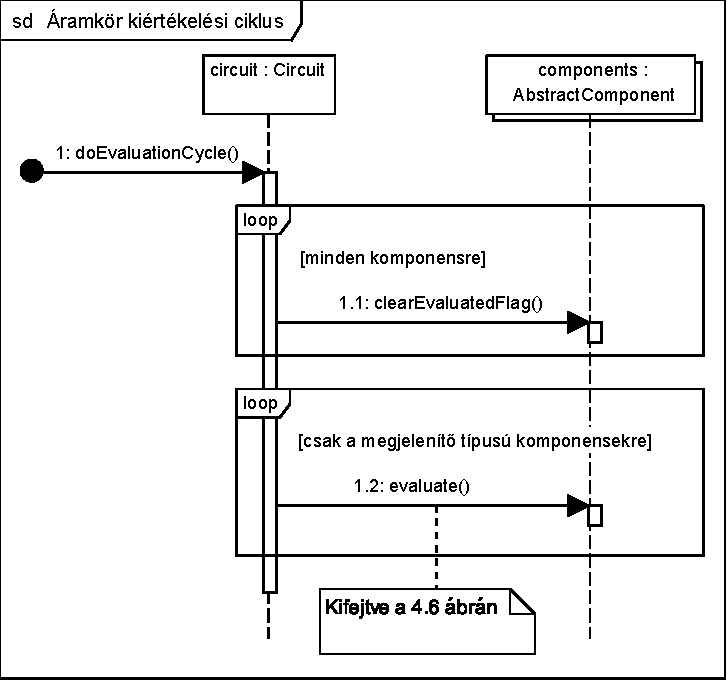
\includegraphics{chapters/chapter04/seqdiagrams/new/doEvalCycle.pdf}
\caption{Áramkör kiértékelési ciklus}
\label{fig:circuit_sim}
\end{center}
\end{figure}

\begin{figure}[H]
\begin{center}
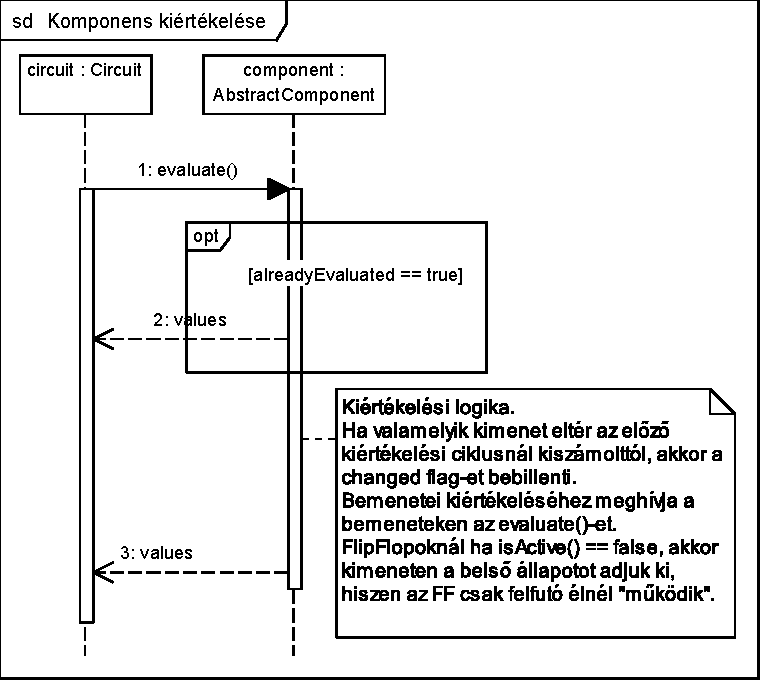
\includegraphics{chapters/chapter04/seqdiagrams/new/evaluate.pdf}
\caption{Komponens kiértékelése}
\label{fig:evaluate}
\end{center}
\end{figure}

\begin{figure}[H]
\begin{center}
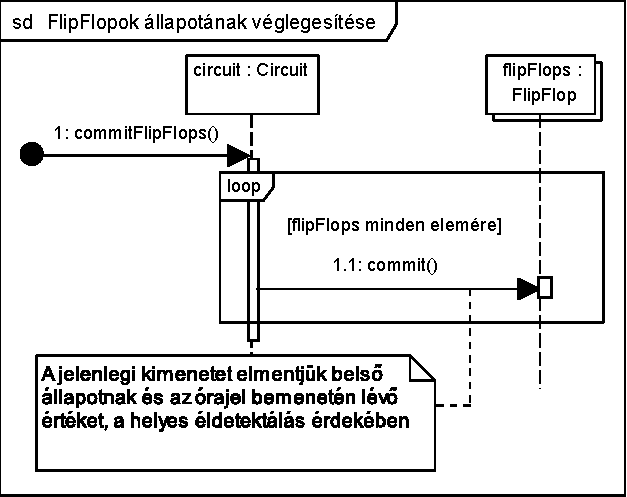
\includegraphics{chapters/chapter04/seqdiagrams/new/commitFlipFlops.pdf}
\caption{Flipflopok állapotának véglegesítése}
\label{fig:commitFlipFlops}
\end{center}
\end{figure}

\begin{figure}[H]
\begin{center}
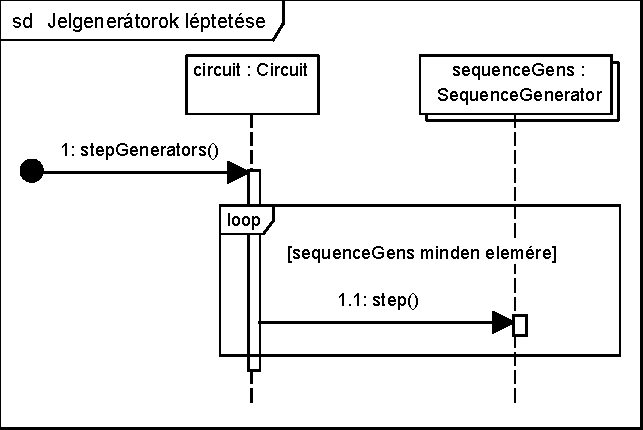
\includegraphics{chapters/chapter04/seqdiagrams/new/stepGenerators.pdf}
\caption{Jelgenerátorok léptetése}
\label{fig:step_gens}
\end{center}
\end{figure}

\begin{figure}[H]
\begin{center}
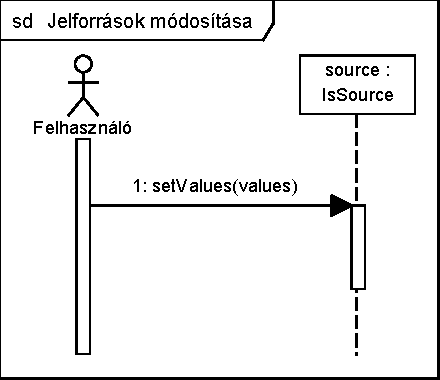
\includegraphics{chapters/chapter04/seqdiagrams/jelforrasok_modositasa.pdf}
\caption{Jelforrások módosítása}
\label{fig:jelforrasok_modositasa}
\end{center}
\end{figure}

\section{State-chartok}

\begin{figure}[H]
\begin{center}
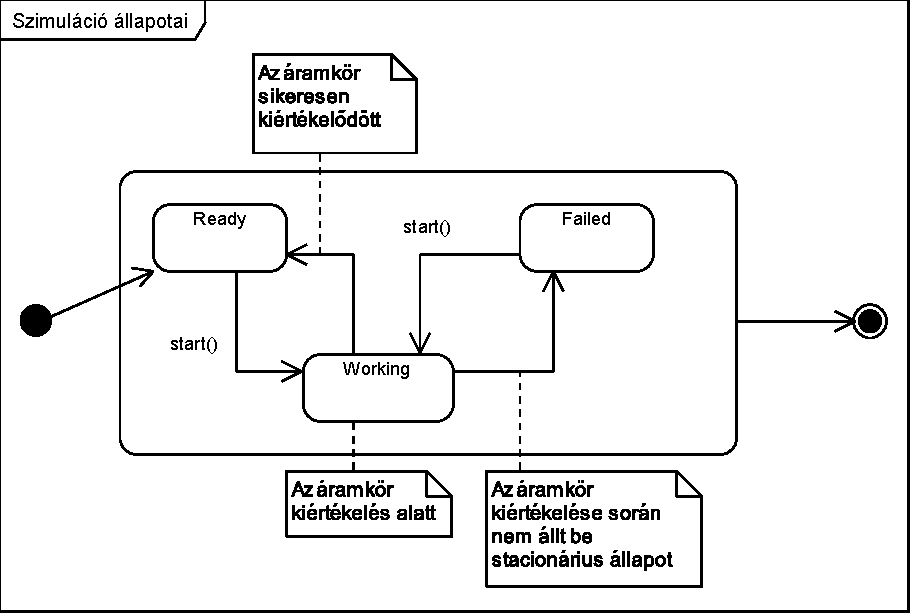
\includegraphics{chapters/chapter04/seqdiagrams/allapotgep.pdf}
\caption{Szimuláció állapotgépe}
\label{fig:allapotgep}
\end{center}
\end{figure}

%\begin{figure}[h]
%\begin{center}
%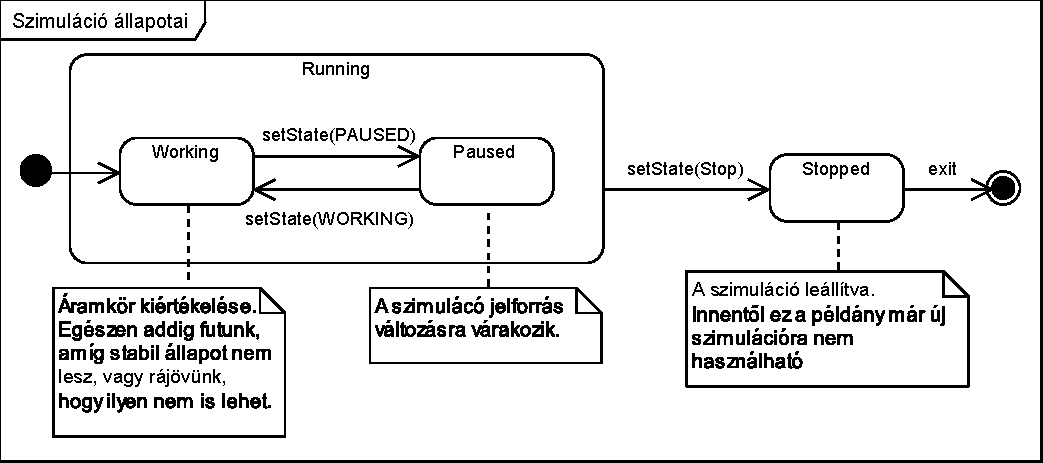
\includegraphics[width=17cm]{chapters/chapter03/seqdiagrams/sim_states.pdf}
%\caption{Szimuláció állapotai}
%\label{fig:sim_states}
%\end{center}
%\end{figure}

